\documentclass{article}

%Page format
\usepackage{pdfpages}
\usepackage{fancyhdr}
\usepackage[margin=1in]{geometry}

%Math packages and custom commands
\usepackage{algpseudocode}
\usepackage{amsthm}
\usepackage{framed}
\usepackage{hyperref}
\usepackage{tikz}
\usepackage[utf8]{inputenc}
\usepackage[margin=1in]{geometry}
\usepackage{mathtools,amsthm}
\usepackage{enumitem,amssymb}
\newtheoremstyle{case}{}{}{}{}{}{:}{ }{}
\theoremstyle{case}
\newtheorem{case}{Case}
\DeclareMathOperator{\R}{\mathbb{R}}
\DeclareMathOperator{\E}{\mathbb{E}}
\DeclareMathOperator{\Var}{\text{Var}}
\DeclareMathOperator{\Cov}{\text{Cov}}
\newcommand{\bvec}[1]{\mathbf{#1}}
\renewcommand{\P}{\mathbb{P}}
\newcommand{\norm}[2][2]{\| #2\|_{#1}}

\definecolor{shadecolor}{gray}{0.9}

\theoremstyle{definition}
\newtheorem*{answer}{Answer}
\newcommand{\note}[1]{\noindent{[\textbf{NOTE:} #1]}}
\newcommand{\hint}[1]{\noindent{[\textbf{HINT:} #1]}}
\newcommand{\recall}[1]{\noindent{[\textbf{RECALL:} #1]}}
\newcommand{\expect}[1]{\noindent{[\textbf{What we expect:} #1]}}
\newcommand{\mysolution}[1]{\noindent{\begin{shaded}\textbf{Your Solution:}\ #1 \end{shaded}}}

\newlist{todolist}{itemize}{2}
\setlist[todolist]{label=$\square$}
\usepackage{pifont}
\newcommand{\cmark}{\ding{51}}%
\newcommand{\xmark}{\ding{55}}%
\newcommand{\done}{\rlap{$\square$}{\raisebox{2pt}{\large\hspace{1pt}\cmark}}%
\hspace{-2.5pt}}
\newcommand{\wontfix}{\rlap{$\square$}{\large\hspace{1pt}\xmark}}


\title{\textbf{CS236 Fall 2023: Deep Generative Models} \\Homework 2}
\date{}

\chead{Homework 2}
\rhead{\today}
\lfoot{}
\cfoot{CS236: Deep Generative Models --- Fall 2023}
\rfoot{\thepage}
\renewcommand{\headrulewidth}{0.4pt}
\renewcommand{\footrulewidth}{0.4pt}
\pagestyle{fancy}
\setlength{\parindent}{0pt}

\begin{document}

\maketitle

\begin{center}
\begin{tabular}{rl}
Instructor: & Stefano Ermon (ermon@cs.stanford.edu)\\
SUNet ID: & 006676235 \\
Name:  & Anuj Shetty \\Collaborators: & Shrey Verma
\end{tabular}
\end{center}

\textit{By turning in this assignment, I agree by the Stanford honor code and declare
that all of this is my own work.} \\

\section*{Problem 1: Implementing the Variational Autoencoder (VAE) (21 points)}
For this problem we will be using PyTorch to implement the variational autoencoder (VAE) and learn a probabilistic model of the MNIST dataset of handwritten digits. Formally, we observe a sequence of binary pixels \( x \in \{0, 1\}^d \), and let \( z \in \mathbb{R}^k \) denote a set of latent variables. Our goal is to learn a latent variable model \( p_\theta(x) \) of the high-dimensional data distribution \( p_{\text{data}}(x) \).\\


The VAE is a latent variable model that learns a specific parameterization $p_\theta(x) = \int p_\theta(x, z)dz = \int p(z)p_\theta (x|z)dz$. Specifically, the VAE is defined by the following generative process:
\begin{align*}
p(z) &= \mathcal{N}(z|0, I) \\
p_\theta(x|z) &= \text{Bern}(x|f_\theta(z))
\end{align*}
In other words, we assume that the latent variables $z$ are sampled from a unit Gaussian distribution $\mathcal{N}(z|0, I)$. The latent $z$ are then passed through a neural network decoder $f_\theta(\cdot)$ to obtain the logits of the $d$ Bernoulli random variables which model the pixels in each image.\\

Although we would like to maximize the marginal likelihood $p_\theta(x)$, computation of $p_\theta(x) =  \int p(z)p_\theta (x|z)dz$ is generally intractable as it involves integration over all possible values of $z$. Therefore, we posit a variational approximation to the true posterior and perform amortized inference as we have seen in class:
\begin{equation*}
q_\phi(z|x) = \mathcal{N}(z|\mu_\phi(x), \text{diag}(\sigma^2_\phi(x)))
\end{equation*}
Specifically, we pass each image $x$ through a neural network which outputs the mean $\mu_\phi$ and diagonal covariance $\text{diag}(\sigma^2_\phi(x))$ of the multivariate Gaussian distribution that approximates the distribution over latent variables $z$ given $x$. We then maximize the lower bound to the marginal log-likelihood to obtain an expression known as the evidence lower bound (ELBO):
\begin{align*}
\log p_\theta(x) &\geq \text{ELBO}(x; \theta, \phi)= \mathbb{E}_{q_{\phi}(z|x)}[\log p_{\theta}(x|z)] - \text{DKL}(q_{\phi}(z|x)||p(z)))
\end{align*}

\text{Notice that the negation of the ELBO decomposes into two terms:} \\
(1) \text{the reconstruction loss:} - $\mathbb{E}_{q_{\phi}(z|x)}[\log p_{\theta}(x|z)]$, \\
(2) \text{the Kullback-Leibler (KL) term:} \text{DKL}$(q_{\phi}(z|x)||p(z))$, \\
\text{e.g.,} -\text{ELBO} = \text{recon. loss} + \text{KL div.} \\
Hence, VAE learning objective is to minimize the negative ELBO.\\

Your objective is to implement the variational autoencoder by modifying \texttt{utils.py} \text{and} \texttt{vae.py}.

\begin{enumerate}

     \item[1.] \textbf{[6 points]} Implement the reparameterization trick in the function \texttt{sample\_gaussian} of \texttt{utils.py}. Specifically, your answer will take in the mean $m$ and variance $v$ of the Gaussian distribution $q_\phi(z|x)$ and return a sample $z \sim q_\phi(z|x)$.
     \mysolution{
        Refer to code submission. 
    }
    
    \item[2.] \textbf{[6 points]} Next, implement \texttt{negative\_elbo\_bound} in the file \texttt{vae.py}. Several of the functions in \texttt{utils.py} will be helpful, so please check what is provided. Note that we ask for the \emph{negative} ELBO, as PyTorch optimizers \emph{minimize} the loss function. Additionally, since we are computing the negative ELBO over a mini-batch of data $\{x^{(i)}\}_{i=1}^n$, make sure to compute the \emph{average} $-\frac{1}{n} \sum_{i=1}^n \text{ELBO}(x^{(i)}; \theta,  \phi)$ over the mini-batch. Finally, note that the ELBO itself cannot be computed exactly since exact computation of the reconstruction term is intractable. Instead we ask that you estimate the reconstruction term via Monte Carlo sampling
    \[
    -\mathbb{E}_{q_\phi(z|x)}[\log p_\theta(x|z)] \approx - \log p_\theta(x|z^{(1)}),
    \]
    where $z^{(1)} \sim q_\phi(z|x)$ denotes a single sample. The function \texttt{kl\_normal} in \texttt{utils.py} will be helpful. Note: \texttt{negative\_elbo\_bound} also expects you to return the \emph{average} reconstruction loss and \emph{average} KL divergence.
    \mysolution{
        Refer to code submission. 
    }

    \item[3.] \textbf{(3 points)} To test your implementation, run \texttt{python run\_vae.py} to train the VAE. Once the run is complete (20000 iterations), it will output (assuming your implementation is correct): 
    \begin{enumerate}
        \item average negative ELBO,
        \item average KL term, and 
        \item average reconstruction loss as evaluated on a test subset that we have selected.
    \end{enumerate}
    Report the three numbers you obtain as part of the write-up. Since we're using stochastic optimization, you may wish to run the model multiple times and report each metric's mean and corresponding standard error. (Hint: the negative ELBO on the test subset should be somewhere around 100.)
    \mysolution{
    
    % NELBO: 101.3690414428711. KL: 19.087217330932617. Rec: 82.28182220458984
    % NELBO: 101.49286651611328. KL: 19.6041259765625. Rec: 81.88871002197266        
    % NELBO: 102.19031524658203. KL: 19.47098159790039. Rec: 82.71932983398438
    % NELBO: 101.13567352294922. KL: 19.395071029663086. Rec: 81.7406005859375
    \\
    NELBO mean: 101.296 \\ 
    NELBO std: 0.3796 \\
    KL mean: 19.389 \\
    KL std: 0.1659 \\
    Reconstruction loss mean: 82.9071 \\
    Reconstruction loss std: 0.2147 
    }
    \newpage
    \item[4.] \textbf{(3 points)} Visualize 200 digits (generate a single image tiled in a grid of 10 $\times$ 20 digits) sampled from $p_{\theta}(x)$.
   
    \begin{figure}[h]
        \centering
        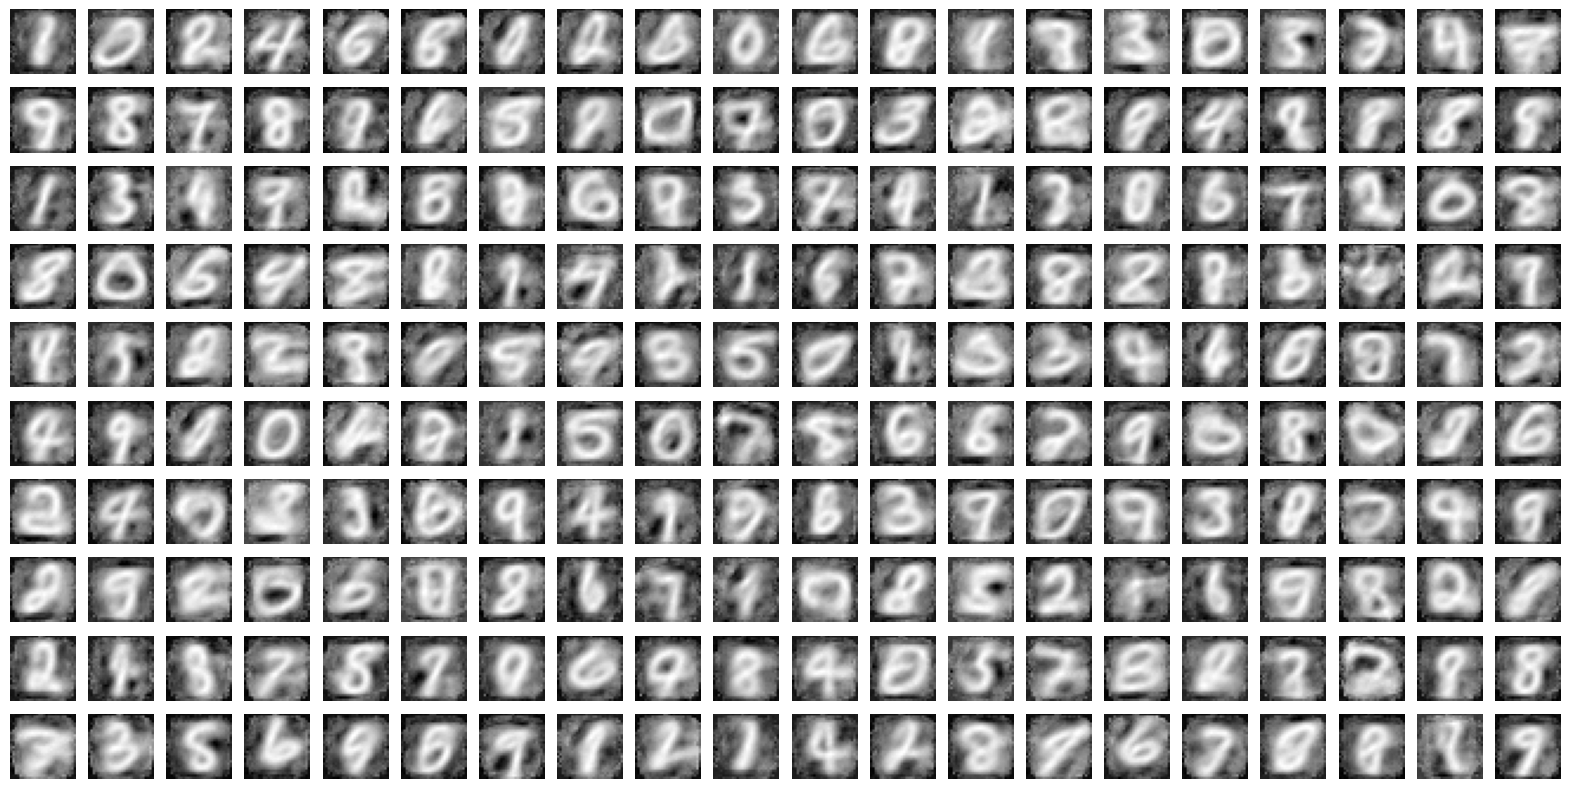
\includegraphics[width=\linewidth]{vae_200_digits.PNG}
        %\caption{Graphical model for SSVAE. Gray nodes denote observed variables.}
        \label{fig:enter-label}
    \end{figure}

    
    \item[5.] \textbf{(3 points)} A popular variation of the normal VAE is called the $\beta$-VAE. The $\beta$-VAE optimizes the following objective:
    \[
    \mathbb{E}_{q_{\phi}(z|x)}[\log p_{\theta}(x|z)] - \beta \text{DKL}(q_{\phi}(z|x)||p(z)))
    \]
    Here, $\beta$ is a positive real number. Offer an intuitive interpretation of the impact of $\beta$ on the optimization of the VAE; specifically, what happens when $\beta = 1$? How about when $\beta$ is increased above 1? For this question, a qualitative description will suffice.
    \mysolution{
        When $\beta=1$, the objective function of the $\beta$-VAE becomes the standard VAE objective. \\
        As $\beta$ is increased above 1, the VAE puts more emphasis on minimizing the KL divergence over the reconstruction error. 
        This will force the latent representations to be more regularized and more distinct. However this can also lead to less accurate reconstruction, since reconstruction loss is given less weightage.
    }
\end{enumerate}


\newpage
\section*{Problem 2: Implementing the Mixture of Gaussians VAE (GMVAE) (22 points)}

Recall that in Problem 1, the VAE's prior distribution was a parameter-free isotropic Gaussian $p(z) = \mathcal{N}(z|0, I)$. While this original setup works well, there are settings in which we desire more expressivity to better model our data. In this problem we will implement the GMVAE, which has a mixture of Gaussians as the prior distribution. Specifically:

\[
p_{\theta}(z) = \sum_{i=1}^{k} \frac{1}{k} \mathcal{N}(z|\mu_i, \text{diag}(\sigma^2_i))
\]

where $i \in \{1, \dots, k\}$ denotes the $i^{th}$ cluster index. For notational simplicity, we shall subsume our mixture of Gaussian parameters $\{\mu_i, \sigma_i\}_{i=1}^k$ into our generative model parameters $\theta$. For simplicity, we have also assumed fixed uniform weights $\frac{1}{k}$ over the possible different clusters. Apart from the prior, the GMVAE shares an identical setup as the VAE:

\[
q_{\phi}(z|x) = \mathcal{N}(z|\mu_{\phi}(x), \text{diag}(\sigma^2_{\phi}(x))
\]

\[
p_{\theta}(x|z) = \text{Bern}(x|f_{\theta}(z))
\]

Although the ELBO for the GMVAE: $\mathbb{E}_{q_{\phi}(z)}[\log p_{\theta}(x|z)] - \text{DKL}(q_{\phi}(z|x)||p(z))$ is identical to that of the VAE, we note that the KL term $\text{DKL}(q_{\phi}(z|x)||p(z))$ cannot be computed analytically between a Gaussian distribution $q_{\phi}(z|x)$ and a mixture of Gaussians $p_{\theta}(z)$. However, we can obtain its unbiased estimator via Monte Carlo sampling:

\[
\text{DKL}(q_{\phi}(z|x)||p_\theta(z)) \approx \log q_{\phi}(z^{(1)}|x) - \log p_{\theta}(z^{(1)})
\]

\[
= \log \mathcal{N}(z^{(1)}|\mu_{\phi}(x), \text{diag}(\sigma^2_{\phi}(x)) - \log \sum_{i=1}^{k} \frac{1}{k} \mathcal{N}(z^{(1)}|\mu_i, \text{diag}(\sigma^2_i))
\],

where $z^{(1)} \sim q_{\phi}(z|x)$ denotes a single sample.

\begin{enumerate}
    \item[1.] \textbf{[16 points]} Implement the (1) log\_normal and (2) log\_normal\_mixture functions in utils.py, and the function negative\_elbo\_bound in gmvae.py. The function log\_mean\_exp in utils.py will be helpful for this problem in ensuring that your implementation is numerically stable.
    \mysolution{
      Refer to code submission.  
    }
    
    \item[2.] \textbf{[3 points]} To test your implementation, run \texttt{python run\_gmvae.py} to train the GMVAE. Once the run is complete (20000 iterations), it will output: the average (1) negative ELBO, (2) KL term, and (3) reconstruction loss as evaluated on a test subset that we have selected. Report the three numbers you obtain as part of the write-up. Since we're using stochastic optimization, you may wish to run the model multiple times and report each metric's mean and the corresponding standard error. (Hint: the negative ELBO on the test subset should be somewhere around 97-99.)

    \mysolution{
        % NELBO: 98.80220031738281. KL: 19.297779083251953. Rec: 79.50442504882812
        % NELBO: 99.95721435546875. KL: 19.749418258666992. Rec: 80.2077865600586
        % NELBO: 99.33302307128906. KL: 19.31629753112793. Rec: 80.0167236328125
        % NELBO: 98.76531982421875. KL: 19.552961349487305. Rec: 79.21237182617188
        \\
        NELBO mean: 99.214 \\ 
        NELBO std: 0.451 \\
        KL mean: 19.479 \\
        KL std: 0.177 \\
        Reconstruction loss mean: 80.735 \\
        Reconstruction loss std: 0.267 \\
    }

    \item[3.] \textbf{[3 points]} Visualize 200 digits (generate a single image tiled in a grid of 10 x 20 digits) sampled from $p_{\theta}(x)$.

    \begin{figure}[h]
        \centering
        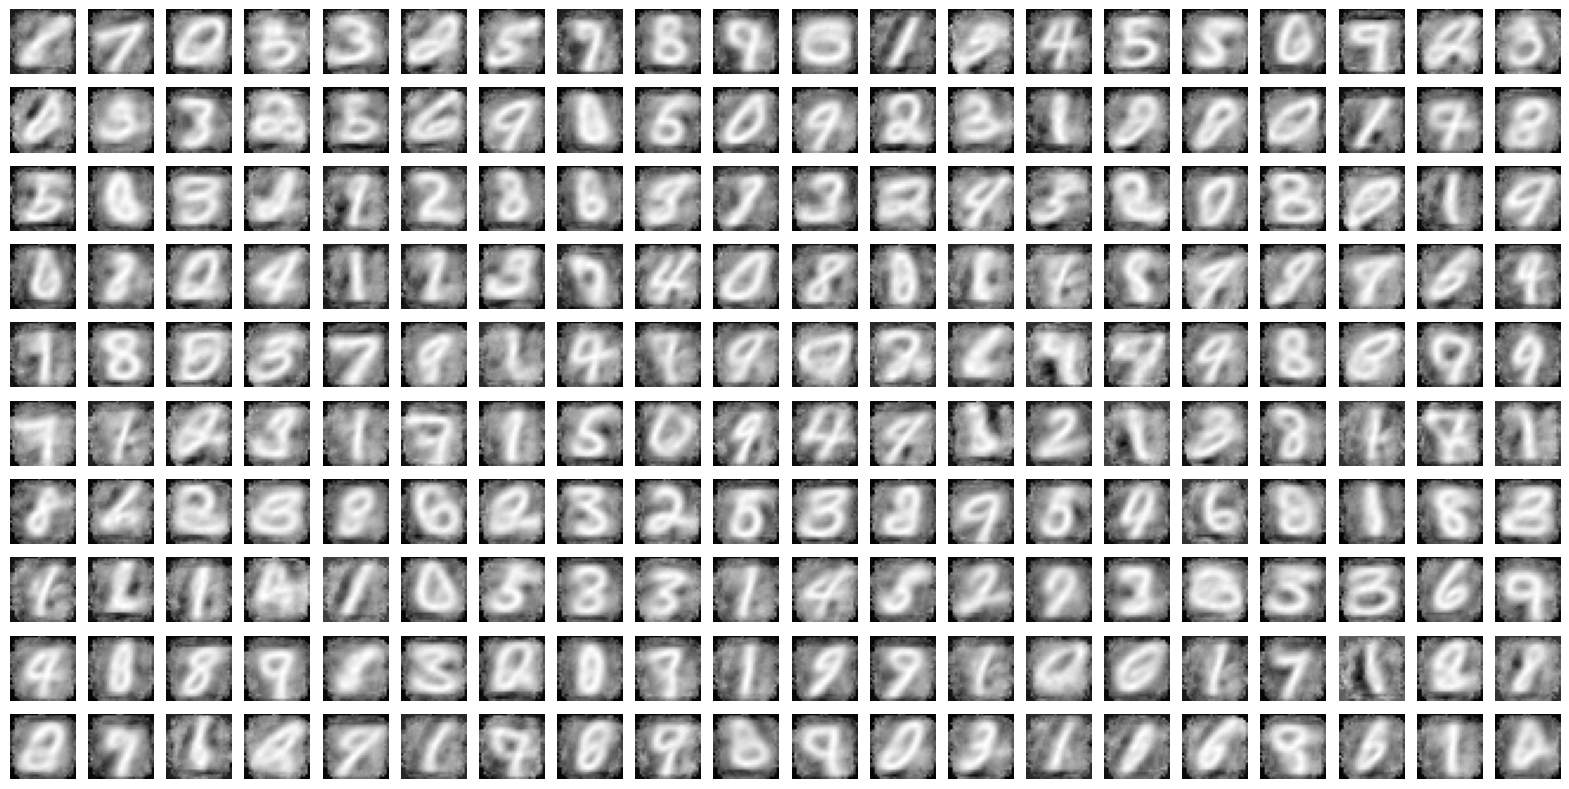
\includegraphics[width=\linewidth]{gmvae_200_digits.PNG}
        %\caption{Graphical model for SSVAE. Gray nodes denote observed variables.}
        \label{fig:enter-label}
    \end{figure}
\end{enumerate}

\newpage
\section*{Problem 3: Implementing the Importance Weighted Autoencoder (IWAE) (21 points)}

While the ELBO serves as a lower bound to the true marginal log-likelihood, it may be loose if the variational posterior $q_{\phi}(z|x)$ is a poor approximation to the true posterior $p_{\theta}(z|x)$. It is worth noting that, for a fixed choice of $x$, the ELBO is, in expectation, the log of the unnormalized density ratio

\begin{align*}
\frac{p_{\theta}(x, z)}{q_{\phi}(z|x)} &= \frac{p_{\theta}(z|x) \cdot p_{\theta}(x)}{q_{\phi}(z|x)}
\end{align*}

where $z \sim q_{\phi}(z|x)$. As can be seen from the RHS, the density ratio is \textit{unnormalized} since the density ratio is multiplied by the constant $p_{\theta}(x)$. We can obtain a tighter bound by averaging multiple unnormalized density ratios. This is the key idea behind IWAE, which uses $m > 1$ samples from the approximate posterior $q_{\phi}(z|x)$ to obtain the following IWAE bound:

\begin{align*}
L_{m}(x; \theta, \phi) &= \mathbb{E}_{z^{(1)},...,z^{(m)}\sim q_{\phi}(z|x)} \left( \log \frac{1}{m} \sum_{i=1}^{m} \frac{p_{\theta}(x, z^{(i)})}{q_{\phi}(z^{(i)}|x)} \right)
\end{align*}

Notice that for the special case of $m = 1$, the IWAE objective $L_{m}$ reduces to the standard ELBO $L_{1} = \mathbb{E}_{z\sim q_{\phi}(z|x)} \left( \log \frac{p_{\theta}(x,z)}{q_{\phi}(z|x)} \right)$.

\begin{enumerate}
    \item[1.] \textbf{[6 points]} Prove that IWAE is a valid lower bound of the log-likelihood, and that the ELBO lower bounds IWAE
    \begin{align*}
    \log p_{\theta}(x) \geq L_{m}(x) \geq L_{1}(x)
    \end{align*}
    for any $m \geq 1$. [Hint: consider Jensen's Inequality]
    \mysolution{
        Jensen's Inequality states that for a concave function $f(x)$, we have $f(\mathbb{E}[x]) &\geq \mathbb{E}[f(x)]$ \\
        We can apply this to the IWAE bound as follows: \\
    \begin{align*}
        
        \log p_{\theta}(x) &= \log \mathbb{E}_{z^{(1)},...,z^{(m)}\sim q_{\phi}(z|x)} \left( \frac{1}{m} \sum_{i=1}^{m} \frac{p_{\theta}(x, z^{(i)})}{q_{\phi}(z^{(i)}|x)} \right) \\
            &\geq \mathbb{E}_{z^{(1)},...,z^{(m)}\sim q_{\phi}(z|x)} \left( \log \frac{1}{m} \sum_{i=1}^{m} \frac{p_{\theta}(x, z^{(i)})}{q_{\phi}(z^{(i)}|x)} \right) \\
        \log p_{\theta}(x) &= L_{m}(x) \\
    \end{align*}
    Thus, we have shown that IWAE is a valid lower bound of the log-likelihood. \\
    Now, we will show that the ELBO lower bounds IWAE. Using Jensen's inequality on the term inside the expectation, with log as the concave function, we get:\\
    \begin{align*}
        \frac{1}{m} \sum_{i=1}^{m} \log \left(\frac{p_{\theta}(x, z^{(i)})}{q_{\phi}(z^{(i)}|x)} \right) &\leq \log \left( \frac{1}{m} \sum_{i=1}^{m} \frac{p_{\theta}(x, z^{(i)})}{q_{\phi}(z^{(i)}|x)}\right) \\
        \mathbb{E}_{z^{(1)},...,z^{(m)}\sim q_{\phi}(z|x)} \left( \frac{1}{m} \sum_{i=1}^{m} \log \left(\frac{p_{\theta}(x, z^{(i)})}{q_{\phi}(z^{(i)}|x)} \right) \right) &\leq \mathbb{E}_{z^{(1)},...,z^{(m)}\sim q_{\phi}(z|x)} \left( \log \left( \frac{1}{m} \sum_{i=1}^{m} \frac{p_{\theta}(x, z^{(i)})}{q_{\phi}(z^{(i)}|x)}\right) \right) \\
        \frac{1}{m} \sum_{i=1}^{m} \log \left( \mathbb{E}_{z^{(1)},...,z^{(m)}\sim q_{\phi}(z|x)} \left( \frac{p_{\theta}(x, z^{(i)})}{q_{\phi}(z^{(i)}|x)} \right) \right) &\leq L_{m}(x; \theta, \phi) \\
        \log \left( \mathbb{E}_{z^{(1)},...,z^{(m)}\sim q_{\phi}(z|x)} \left( \frac{p_{\theta}(x, z^{(i)})}{q_{\phi}(z^{(i)}|x)} \right) \right) &\leq L_{m}(x; \theta, \phi) \\
        L_{1}(x; \theta, \phi) &\leq L_{m}(x; \theta, \phi)
    \end{align*}
    This shows that IWAE is lower bounded by the ELBO. Thus proved.
    }
    
    \item[2.] \textbf{[6 points]} Implement IWAE for VAE in the \texttt{negative\_iwae\_bound} function in \texttt{vae.py}. The functions \texttt{duplicate} and \texttt{log\_mean\_exp} defined in \texttt{utils.py} will be helpful.
    \mysolution{
        Refer to code submission. 
    }
    
    \item[3.] \textbf{[3 points]} Run \texttt{python run\_vae.py --train 0} to evaluate your implementation against the test subset. This will output IWAE bounds for $m = \{1,10,100,1000\}$. Check that the IWAE-1 result is consistent with your reported ELBO for the VAE. Report all four IWAE bounds for this write-up.
    \mysolution{
        Negative IWAE-1: 101.29 \\
        Negative IWAE-10: 98.18 \\
        Negative IWAE-100: 97.63 \\
        Negative IWAE-1000: 97.53 
    }
    
    \item[4.] \textbf{[6 points]} As IWAE only requires the averaging of multiple unnormalized density ratios, the IWAE bound is also applicable to the GMVAE model. Repeat parts 2 and 3 for the GMVAE by implementing the \texttt{negative\_iwae\_bound} function in \texttt{gmvae.py}. Compare and contrast IWAE bounds for GMVAE and VAE.
    \mysolution{
        Negative IWAE-1: 100.82 \\
        Negative IWAE-10: 98.19 \\
        Negative IWAE-100: 97.07 \\
        Negative IWAE-1000: 96.97 
    }
\end{enumerate}

\newpage
\section*{Problem 4: Implementing the Semi-Supervised VAE (SSVAE) (19 points)}

So far we have dealt with generative models in the unsupervised setting. We now consider semi-supervised learning on the MNIST dataset, where we have a small number of labeled $x_\ell=\{(x^{(i)}, y^{(i)})\}_{i=1}^{100}$ pairs in our training data and a large amount of unlabeled data and a large amount of unlabeled data $x_u=\{x^{(i)}\}^{60000}_{i=101}$. A label $y^{(i)}$ for an image is simply the number the image $x^{(i)}$ represents. We are interested in building a classifier that predicts the label y given the
sample x. One approach is to train a classifier using standard approaches using only the labeled data. However, we would like to leverage the large amount of unlabeled data that we have to improve our classifier's performance.\\

We will use a latent variable generative model (VAE), where the labels $y$ are partially observed, and $z$ are always unobserved. The benefit of a generative model is that it allows us to naturally incorporate unlabeled data into the maximum likelihood objective function, simply by marginalizing $y$ when it is unobserved. We will implement the Semi-Supervised VAE (SSVAE) for this task, which follows the generative process specified below:

\begin{align*}
p(z) &= \mathcal{N}(z|0,I) \\
p(y) &= \text{Categorical}(y|\pi)=\frac{1}{10} \\
p(x|y,z) &= \text{Bern}(x|f_\theta(y,z))
\end{align*}

where $\pi = (1/10, \dots ,1/10)$ is a fixed uniform prior over the 10 possible labels and each sequence of pixels $x$ is modeled by a Bernoulli random variable parameterized by the output of a neural network decoder $f_\theta$ ($\cdot$).

\begin{figure}[h]
    \centering
    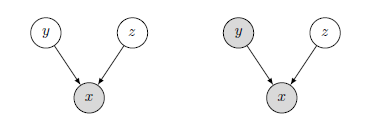
\includegraphics[width=0.5\linewidth]{fig.PNG}
    \caption{Graphical model for SSVAE. Gray nodes denote observed variables; unshaded nodes denote latent variables. Left: SSVAE for the setting where the labels $y$ are unobserved; Right: SSVAE where some data points $(x,y)$ have observed labels.}
    \label{fig:enter-label}
\end{figure}

To train a model on the datasets $X_\ell$ and $X_u$, the principle of maximum likelihood suggests that we find the model $p_\theta$ which maximizes the likelihood over both datasets. Assuming the samples from $X_l$ and $X_u$ are drawn i.i.d., this translates to the following objective:

\begin{align*}
\max_\theta \sum_{x \in X_u} \log p_\theta(x) + \sum_{x,y \in X_\ell} \log p_\theta(x,y)
\end{align*}

where 
\[ p_\theta(x) = \sum_{y \in \mathcal{Y}} \int p_\theta(x, y, z) dz \]
\[ p_\theta(x, y) = \int p_\theta(x, y, z) dz. \]

To overcome the intractability of exact marginalization of the latent variables \( z \), we will instead maximize their respective evidence lower bounds,
\[ \max_{\theta, \phi} \sum_{x \in X_u} \text{ELBO}(x; \theta, \phi) + \sum_{x, y \in \mathcal{X}} \text{ELBO}(x, y; \theta, \phi), \]

where we introduce some amortized inference model \( q_{\phi}(y, z|x) = q_{\phi}(y|x)q_{\phi}(z|x, y) \). Specifically,
\[ q_{\phi}(y|x) = \text{Categorical}(y|f_{\phi}(x)) \]
\[ q_{\phi}(z|x, y) = \mathcal{N}(z|\mu_{\phi}(x, y), \text{diag}(\sigma^2_{\phi}(x, y))). \]

where the parameters of the Gaussian distribution are obtained through a forward pass of the encoder. We note that $q_\phi(y|x) = \text{Categorical}(f_\phi(x))$ 
is actually an MLP classifier that is also a part of the inference model, and it predicts the probability of the label $y$ given the observed data $x$. \\

We use this amortized inference model to construct the ELBOs:
\[ ELBO(x; \theta, \phi) = \mathbb{E}_{q_\phi(y,z|x)} \left[ \log \frac{p_\theta(x, y, z)}{q_\phi(y,z|x)} \right] \]
\[ ELBO(x, y; \theta, \phi) = \mathbb{E}_{q_\phi(z|x,y)} \left[ \log \frac{p_\theta(x, y, z)}{q_\phi(z|x, y)} \right] \]

However, Kingma et al. (2014) observed that maximizing the lower bound of the log-likelihood is not sufficient to learn a good classifier. Instead, they proposed to introduce an additional training signal that directly trains the classifier on the labeled data.

\begin{equation}
\max_{\theta, \phi}  \sum_{x \in X_u} \text{ELBO}(x; \theta, \phi) + \sum_{x, y \in X_\ell} \text{ELBO}(x, y; \theta, \phi) + \alpha \sum_{x, y \in X_\ell} \log q_{\phi}(y|x) 
\end{equation}
where \( \alpha \geq 0 \) weights the importance of the classification accuracy. In this problem, we will consider a simpler variant of this objective that works just as well in practice,
\begin{equation}
\max_{\theta, \phi} \sum_{x \in X} \text{ELBO}(x; \theta, \phi) + \alpha \sum_{x, y \in X_\ell} \log q_{\phi}(y|x)
\end{equation}

where $X = \{X_u, X_\ell\}$. It is worth noting that the introduction of the classification loss has a natural interpretation as maximizing the ELBO subject to the soft constraint that the classifier $q_\phi(y|x)$ (which is a component of the amortized inference model) achieves good performance on the labeled dataset. This approach of controlling the generative model by constraining its inference model is thus a form of amortized inference regularization.

\begin{enumerate}
    \item [1.] \textbf{[1 point]} Run python \texttt{run\_ssvae.py --gw} 0. The \texttt{gw} flag denotes how much weight to put on the \texttt{ELBO(x)} term in the objective function; scaling the term by zero corresponds to a traditional supervised learning setting on the small labeled dataset only, where we ignore the unlabeled data. Report your classification accuracy on the test set after the run completes (30000 iterations).
    \mysolution{
        Test set classification accuracy: 0.7312999963760376
    }

    \item[2.] \textbf{[15 points]} Implement the \texttt{negative\_elbo\_bound} function in \texttt{ssvae.py}. Note that the function expects as output the negative Evidence Lower Bound as well as its decomposition into the following terms,
    \begin{align}
    -\text{ELBO}(x; \theta, \phi) &= \mathbb{E}_{q_{\phi}(y|x)} \left[ \log \frac{p(y)}{q_{\phi}(y|x)} \right] - \mathbb{E}_{q_{\phi}(y|x)}\mathbb{E}_{q_{\phi}(z|x,y)} \left[ \log \frac{p(z)}{q_{\phi}(z|x, y)} + \log p_\theta(x|z, y) \right] \\
    &= \text{D}_{KL}\left(q_{\phi}(y|x) || p(y)\right) + \mathbb{E}_{q_{\phi}(y|x)}\left[\text{D}_{KL}\left(q_{\phi}(z|x, y) || p(z)\right)\right] + \mathbb{E}_{q_{\phi}(y,z|x)} \left[ -\log p_\theta(x|z, y) \right].
    \end{align}

    Since there are only ten labels, we shall compute the expectations with respect to $q_{\phi}(y|x)$ exactly, while using a single Monte Carlo sample of the latent variables z sampled from $q_{\phi}(z|x,y)$ when dealing with the reconstruction term. In other words, we approximate the negative ELBO with
    \[ 
    D_{KL}(q_{\phi}(y|x) || p(y)) + \sum_{y \in \mathcal{Y}} q_{\phi}(y|x) \left[ D_{KL}(q_{\phi}(z|x,y) || p(z) - log p_{\theta}(x|y^{(y)},z)) \right],
    \]
    where $z^{(y)} \sim q_{\phi}(z|x,y)$ denotes a sample from the inference distribution when conditioned on a possible $(x,y)$ pairing. The functions \texttt{kl\_normal} and \texttt{kl\_cat} in \texttt{utils.py} will be useful.
    \mysolution{
        Refer to code submission. 
    }

    \item[3.] \textbf{[3 points]} Run \texttt{python run\_ssvae.py}. This will run the SSVAE with the ELBO(x) term included, and thus perform semi-supervised learning. Report your classification accuracy on the test set after the run completes.
    \mysolution{
        Test set classification accuracy: 0.1728000044822693  :$\left($
    }
    
\end{enumerate}
\newpage


\section*{Bonus: Style and Content Disentanglement in SVHN (9 points)}

A curious property of the SSVAE graphical model is that, in addition to the latent variables \(y\) learning to encode the content (i.e. label) of the image, the latent variables \(z\) also learns to encode the style of the image. We shall demonstrate this phenomenon on the SVHN dataset. To make the problem simpler, we will only consider the fully-supervised scenario where \(y\) is fully-observed. This yields the fully-supervised VAE, shown below.

\begin{figure}[h]
    \centering
    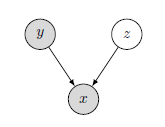
\includegraphics[width=0.3\linewidth]{fig2.PNG}
    \caption{Graphical model for SSVAE. Gray nodes denote observed variables.}
    \label{fig:enter-label}
\end{figure}

\begin{enumerate}
    \item[1.] \textbf{[3 points]} Since fully-supervised VAE (FSVAE) always conditions on an observed \(y\) in order to generate the sample \(x\), it is a \textit{conditional} variational autoencoder. Derive the Evidence Lower Bound ELBO(\(x; \theta, \phi, y\)) of the conditional log probability \(\log p_{\theta}(x|y)\). You are allowed to introduce the amortized inference model \(q_{\phi}(z|x, y)\).
    \mysolution{
        
    \begin{align}
        \log p_\theta(x|y) &= \log \int p_\theta(x, z|y) dz \\
        &= \log \int p_\theta(x|z, y) p_\theta(z) dz \\
        &= \log \int q_\phi(z|x, y)  \left( \frac{p_\theta(x|z, y) p_\theta(z)}{q_\phi(z|x, y)} \right) dz \\
        &\geq \int q_\phi(z|x, y) \log \left( \frac{p_\theta(x|z, y) p_\theta(z)}{q_\phi(z|x, y)} \right) dz & \text{(Using Jensen's inequality)} \\
        &= \mathbb{E}_{q_\phi(z|x, y)} \left[ \log p_\theta(x|z, y) + \log p_\theta(z) - \log q_\phi(z|x, y) \right] \\
        &= \mathbb{E}_{q_\phi(z|x, y)} \left[ \log p_\theta(x|z, y)\right] - D_{KL} (q_\phi(z|x, y) || p_\theta(z))  \\
        &= \text{ELBO}(x, y; \theta, \phi).
        \end{align}
        
    }
    
    \item[2.] \textbf{[6 points]} Implement the \texttt{negative\_elbo\_bound} function in \texttt{fsvae.py}. In contrast to the MNIST dataset, the SVHN dataset has a \textit{continuous} observation space
    
    \begin{align*}
        p(z) &= \mathcal{N}(z|0, I) \\
        p_{\theta}(x|y, z) &= \mathcal{N}(x|\mu_{\theta}(y, z), \text{diag}(\sigma^2_{\theta}(y, z))).
    \end{align*}
    
    To simplify the problem more, we shall assume that the \textit{variance} is fixed at
    
    \[
    \text{diag}(\sigma^2_{\theta}(y, z)) = \frac{1}{10}I
    \]
    
    and only train the decoder mean function \(\mu_{\theta}\). Once you have implemented \texttt{negative\_elbo\_bound}, run python \texttt{run\_fsvae.py}. The default settings will use a max iteration of 1 million. We suggest checking the image quality of clip(\(\mu_{\theta}(y, z)\) -- where clip ($\cdot$) performs element-wise clipping of outputs outside the range [0,1] -- every 10k iteration and stopping the training whenever the digit classes are recognizable.
    
    Once you have learned a sufficiently good model, generate twenty latent variables \(z^{(0)}, \dots, z^{(19)} \sim p(z)\). Then, generate 200 SVHN digits (a single image tiled in a grid of 10 x 20 digits) where the digit in the \(i^{th}\) row, \(j^{th}\) column (assuming zero-indexing) is the image \texttt{clip}(\(\mu_{\theta}(y = i, z = j)\)).
    \mysolution{
        
    }
\end{enumerate}

Programming Submission Instruction

See the included README in the programming assignment.

\end{document}
